


\chapter{Overview} \label{Overview}

JavaGroups is toolkit for reliable group communication. Processes can join a group,
send messages to all members or single members and receive messages from members in
the group. The system keeps track of the members in every group, and notifies group
members when a new member joins, or an existing member leaves or crashes. A group
is identified by its name. Groups do not have to be created explicitly; when a
process joins a non-existing group, that group will be created
automatically. Member processes of a group can be located on the same host, within
the same LAN, or across a WAN. A member can be part of multiple groups.


The architecture of JavaGroups is shown in fig. \ref{ArchitectureFig}.


\begin{figure}[htb]
    \center{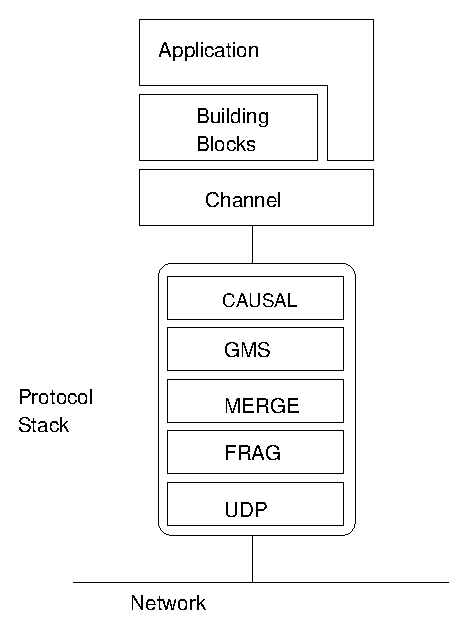
\epsfig{file=figs/Architecture.eps,width=.4\textwidth}}
    \caption{Architecture of JavaGroups}
    \label{ArchitectureFig}
\end{figure}

It consists of 3 parts: (1) the Channel API used by application programmers to
build reliable group communication applications, (2) the building blocks, which are
layered on top of the channel and provide a higher abstraction level and (3) the
protocol stack, which implements the properties specified for a given
channel.

This document describes how to install and {\em use} JavaGroups, ie. the Channel API and
the building blocks. The targeted audience is application programmers who want to use
JavaGroups to build reliable distributed programs that need group
communication. Programmers who want to {\em implement} their own protocols to be used with
JavaGroups should consult the Programmer's Guide for more details about the
architecture and implementation of JavaGroups.

A channel is connected to a protocol stack. Whenever the application sends a message,
the channel passes it on to the protocol stack, which passes it to the topmost
protocol. The protocol processes the message and the passes it on to the protocol
below it. Thus the message is handed from protocol to protocol until the bottom
protocol puts it on the network. The same happens in the reverse direction: the
bottom (transport) protocol listens for messages on the network. When a message is
received it will be handed up the protocol stack until it reaches the channel. The
channel stores the message in a queue until the application consumes it.

When an application connects to the channel, the protocol stack will be started, and
when it disconnects the stack will be stopped. When the channel is closed, the stack
will be destroyed, releasing its resources.

The following three sections give an overview of channels, building blocks and the
protocol stack.



  \section{Channel}

  To join a group and send messages, a process has to create a {\em channel} and
  connect to it using the group name (all channels with the same name form a
  group). The channel is the handle to the group. While connected, a member may
  send and receive messages to/from all other group members. The client leaves a
  group by disconnecting from the channel. A channel can be reused: clients can
  connect to it again after having disconnected. However, a channel allows only 1
  client to be connected at a time. If multiple groups are to be joined, multiple
  channels can be created and connected to. A client signals that it no longer
  wants to use a channel by closing it. After this operation, the channel cannot be
  used any longer.

  Each channel has a unique address. Channels always know who the other members are
  in the same group: a list of member addresses can be retrieved from any
  channel. This list is called a {\em view}. A process can select an address from
  this list and send a unicast message to it (also to itself), or it may send a
  multicast message to all members of the current view. Whenever a process joins or
  leaves a group, or when a crashed process has been detected, a new {\em view} is
  sent to all remaining group members. When a member process is suspected of having
  crashed, a {\em suspicion message} is received by all non-faulty members. Thus,
  channels receive regular messages, view messages and suspicion messages. A client
  may choose to turn reception of views and suspicions on/off on a channel basis.

  Channels are similar to BSD sockets: messages are stored in a channel until a
  client removes the next one (pull-principle). When no message is currently
  available, a client is blocked until the next available message has been
  received.

  A channel can be implemented over a number of alternatives for group
  transport. Therefore, a channel is an abstract class, and concrete implementations
  are derived from it, e.g. a channel implementation using its own protocol stack, or
  others using existing group transports. Currently, JavaGroups offers 2
  implementations of channels: JChannel, which is the default group transport and
  EnsChannel, which is based on Ensemble \cite{Ensemble:1997}, a reliable group
  communication toolkit written in ML. Applications only deal with the abstract
  channel class, and the actual implementation can be chosen at startup
  time\footnote{The most recent version of Ensemble is not supported as the format
  for communication between EnsChannel and Ensemble has changed. Possibly Ensemble
  support will be dropped in one of the next releases unless someone volunteers to
  port EnsChannel to use the latest Ensemble version.}.

  The properties for a channel are specified in a colon-delimited string format.
  When creating a channel (JChannel) a protocol stack will be created according to
  these properties. All messages will pass through this stack, ensuring the quality
  of service specified by the properties string for a given channel.
  
  The Channel API and its related classes is described in \ref{Channel}.



  \section{Building Blocks}
    
  Channels are simple and primitive. They offer the bare functionality of group
  communication, and have on purpose been designed after the simple model of BSD
  sockets, which are widely used and well understood. The reason is that an
  application can make use of just this small subset of JavaGroups, without having to
  include a whole set of sophisticated classes, that it may not even need. Also, a
  somewhat minimalistic interface is simple to understand: a client needs to know
  about 12 methods to be able to create and use a channel (and oftentimes will only
  use 3-4 methods frequently).

  Channels provide asynchronous message sending/reception, somewhat similar to UDP. A
  message sent is essentially put on the network and the send() method will return
  immediately. Conceptual {\em requests}, or {\em responses} to previous requests,
  are received in undefined order, and the application has to take care of matching
  responses with requests.

  Also, an application has to actively {\em retrieve} messages from a channel
  (pull-style); it is not notified when a message has been received. Note that
  pull-style message reception often needs another thread of execution, or some form
  of event-loop, in which a channel is periodically polled for messages.

  JavaGroups offers building blocks that provide more sophisticated APIs on top of a
  Channel. Building blocks either create and use channels internally, or require an
  existing channel to be specified when creating a building block. Applications
  communicate directly with the building block, rather than the channel. Building
  blocks are intended to save the application programmer from having to write tedious
  and recurring code, e.g. request-response correlation.

  Building blocks are described in \ref{BuildingBlocks}.
    


  \section{The Protocol Stack}

  As discussed above, JavaGroups provides two channel implementations: an
  Ensemble-based channel and its own channel based on a Java protocol stack. The
  latter is a protocol stack containing a number of protocol layers in a
  bidirectional list. All messages sent and received over the channel have to pass
  through the protocol stack. Every layer may modify, reorder, pass or drop a
  message, or add a header to a message. A fragmentation layer might break up a
  message into several smaller messages, adding a header with an id to each fragment,
  and re-assemble the fragments on the receiver's side.

  The composition of the protocol stack, i.e. its layers, is determined by the
  creator of the channel: a property string defines the layers to be used (and the
  parameters for each layer). This string might be interpreted differently by each
  channel implementation; in JChannel it is used to create the stack, depending on
  the protocol names given in the property.

  Knowledge about the protocol stack is not necessary when only {\em using}
  channels in an application. However, when an application wishes to ignore the
  default properties for a protocol stack, and configure their own stack, then
  knowledge about what the individual layers are supposed to do is needed. Although
  it is syntactically possible to stack any layer on top of each other (they all
  have the same interface), this wouldn't make sense semantically in most cases.


